\section{A Modular Design Space of LLM Agents}

\begin{figure}[!t]
\vspace{-6.5mm}
\begin{center}
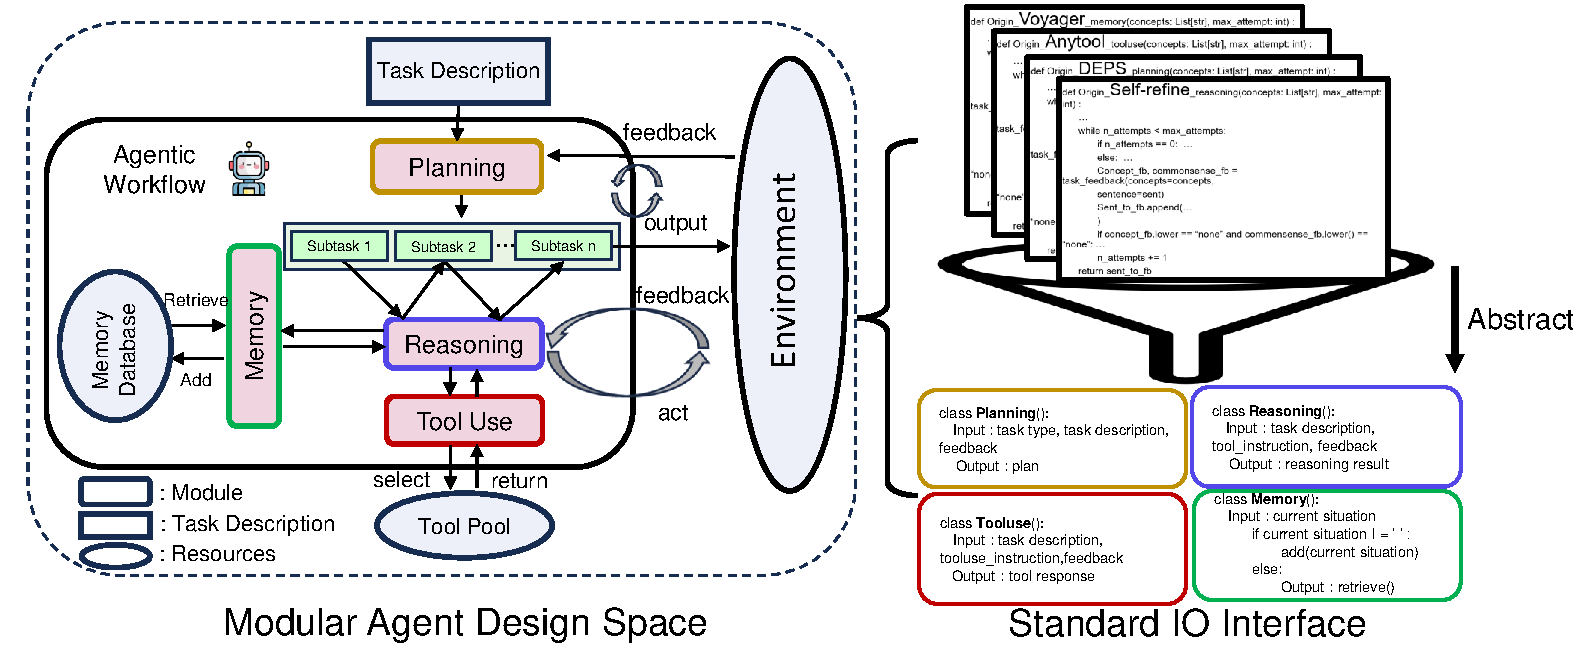
\includegraphics[width=14cm]{Figures/f2.pdf}
\caption{Illustration of the modular agent design space and agentic workflow (left) and the standardized IO interface of four types of modules (right).}
\label{figure2}
\end{center}
\end{figure}

\subsection{Background}

Using LLMs for automatic optimization has been a widely explored topic, such as applications in code generation~\citep{lehman2023evolution,romera2024mathematical} and neural architecture search~\citep{nasir2024llmatic,chen2024evoprompting}.
There are several recent studies that explore the problem of prompting LLMs to design LLM agentic systems. OPRO~\citep{yang2024large} and Promptbreeder~\citep{fernando2024promptbreeder} can be viewed as leveraging the reasoning power of LLMs to improve the prompt of LLM agents. More importantly, ADAS introduces the idea of searching the entire agentic system defined in code space, and propose a Meta Agent Search algorithm that discovers LLM agents outperforming state-of-the-art human designs~\citep{hu2024automated}. Our main difference and contribution lie in introducing a modular design space for LLM agents, which can provide a standard framework to support the convenient reuse of existing successful agent components and fruitful innovative agent module discovery. 

A modular design space for LLM agents facilitates the reuse of prior successful designs and supports the exploration of new architectures. 
At the core of such modularization is the standardization of input-output interfaces, which ensures both extensibility and seamless integration with existing designs.
Many experts in the field have proposed building LLM agentic systems with key modular components from engineering~\citep{weng2023agent} and cognitive perspectives~\citep{sumers2023cognitive}. 
However, these proposals remain largely conceptual, lacking implementable solutions to unify existing LLM agents. Besides, current LLM workflow program frameworks (\emph{e.g.}, LangChain and AutoGPT) only provide operation-level components, which cannot support module-level search that best exploits the potential of prior successful designs.

To address these problems, we perform a comprehensive literature review of publications from NeurIPS, ICML, and ICLR over the past three years. 
The review focuses on papers with the keywords ``LLM'', ``Agent'', or ``Large Language Model'' in their titles while excluding works related to multi-agent systems or agents that require additional training.
Note that our aim is not to propose the most comprehensive, one-for-all LLM agent design space, but to offer a standardized framework that enables the recombination of existing agents and facilitates the discovery of new ones.
As a result, we sort out 16 popular LLM agents and abstract a modular design space with 1050 possible combinations, which can be easily extended when new modules are discovered.
Below, we describe the agentic workflow and the function of four modules in our design space.

\subsection{Workflow overview}
The proposed agent workflow operates through an iterative process with the interconnection of the above four modules, as shown in Figure~\ref{figure2}. 
Upon receiving a task $d$, the agent starts with the \emph{planning} module, decomposing it into $n$ sub-tasks$\{s_1, s_2, \dots, s_n\}$. 
Next, these sub-tasks are passed to the \emph{reasoning} module sequentially.
Taking the sub-task $s_i$ description as input, the \emph{reasoning} module explores to prompt LLMs to give the result.
When reasoning encounters limitations in internal knowledge of LLMs, the \emph{tool use} module is activated to select an appropriate tool from the pre-defined tool pool $\tau$, supporting problem-solving.
Besides, the reasoning process also accesses the \emph{memory} module which reads and writes necessary observations and experiences from a memory database $mem$ to help reasoning.
The reasoning result of each sub-task will be transformed into actions, guiding the agent to interact with the external environment.
% Combined with the received feedback from the environment, the \emph{reasoning} module runs iteratively to refine the reasoning results.
After all sub-tasks are finished or the reasoning process gets stacked, the agent will activate the \emph{planning} module to adjust the plan with the received feedback.
The agent conducts such a trial-and-error loop until the task $d$ is completed or the set maximum trial number is reached.

\textbf{Planning.} 
The planning module is responsible for decomposing the targeted task into smaller sub-tasks. 
Given a task description $d$ and optional feedback information $f$, the planning module $P$ strategically decomposes the targeted task into a sub-task sequence $ \{s_1, s_2, \dots, s_n\} = P(d, f)$.
Such decomposition is critical for handling very complex tasks with long-term characteristics, especially for agents in open-world environments such as MineCraft~\citep{wang2024voyager,wang2024describe}.

\textbf{Reasoning.}
LLMs have exhibited remarkable reasoning abilities under advanced prompting approaches such as CoT~\citep{wei2022chain}, ToT~\citep{yao2024tree}, and SoT~\citep{shang2024defint}, shaping the foundation of the intelligence of LLM agents.
The reasoning module $R$ is invoked to solve the sub-tasks sequentially after planning, which takes each sub-task $s_i$ and optional feedback information $f_i$ as input and outputs a solution $r_i=R(s_i,f_i)$.
% This is usually achieved by diverse prompting approaches for LLMs, such as Chain-of-Thought (CoT) and Tree-of-Thoughts (ToT).

\textbf{Tool use.}
The ability of using external tools~\citep{shen2024hugginggpt,schick2024toolformer} overcomes the limitations of the LLM’s internal knowledge during the reasoning process. 
% This module is designed around \textit{when} to use tools and \textit{how} to select the most appropriate tool. 
% When the reasoning process needs external assistance, the tool use module $T$ will be invoked to select the suitable tool for problem-solving.
Formally, given certain problem $p_{ij}$ derived from the reasoning process of sub-task $s_i$ and a pre-defined tool pool $\tau$, the tooluse module $T$ selects the best-matched tool $t_{ij}$ to address the problem, denoted as $t_{ij} = T(p_{ij}, \tau)$, where $t_{ij} \in \tau$. 

\textbf{Memory.}
Memory plays a critical role by storing past thoughts, actions, and observations of agents~\citep{park2023generative,shinn2024reflexion}.
% These internal logs are dynamically written to and retrieved from the memory, controlled by a reflection module.
During the reasoning process, these internal logs are dynamically written to and retrieved from the memory database $mem$, controlled by the memory module $M$.
The writing process can be expressed as $mem = M_{write}(o, mem)$, where $o$ denotes the current observations. The retrieval process is $m = M_{retrieve}(o, mem)$, where $m$ denotes the retrieved knowledge relevant to the current situation.


